\documentclass[a4paper,11pt]{article}
\usepackage[utf8]{inputenc}
\usepackage[T1]{fontenc}
\usepackage[english]{babel}
\usepackage{lmodern}\usepackage{microtype}
\usepackage{amsmath,amssymb,bm,mathtools}
\usepackage{geometry}
\geometry{a4paper,left=2.3cm,right=2.3cm,top=2.0cm,bottom=2.0cm}
\usepackage{booktabs,array}
\usepackage{xcolor}\definecolor{bokug}{RGB}{0,135,60}
\usepackage{tikz}
\usetikzlibrary{patterns,arrows.meta,calc,decorations.pathmorphing}
\usepackage{fancyhdr}\pagestyle{fancy}
\renewcommand{\headrulewidth}{0.4pt}
\usepackage{enumitem}\setlength{\parindent}{0pt}\setlength{\parskip}{4pt}

\begin{document}
\fancyhead[L]{\small VU Mechanik – LAWI 100515 (PI)}
\fancyhead[R]{\small SS 2026}
\fancyfoot[C]{\thepage}
\begin{center}{\large\bfseries\color{bokug}University of Natural Resources and Life Sciences, Vienna (BOKU)}\\[2pt]{\large\bfseries VU Mechanik – LAWI 100515 (PI)}\\[4pt]Exam \textbf{Group A} \hfill Date: 26.06.2026\\[2pt]\rule{\linewidth}{0.4pt}\end{center}

\textbf{Given system}\\[-2pt]
The system consists of two rigid bodies connected by a hinge at $C$: a bending beam $A$--$C$ (fixed support at $A$) and a truss (roller support at $B$).
\begin{center}
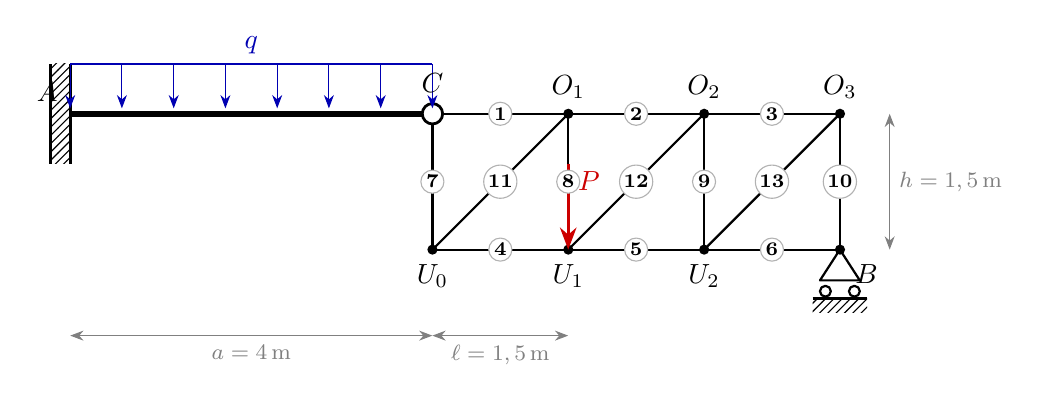
\begin{tikzpicture}[scale=1.15, >=Stealth, line join=round]
  \coordinate (A) at (0.000,0.000);
  \coordinate (C) at (4.000,0.000);
  \coordinate (O1) at (5.500,0.000);
  \coordinate (O2) at (7.000,0.000);
  \coordinate (O3) at (8.500,0.000);
  \coordinate (U0) at (4.000,-1.500);
  \coordinate (U1) at (5.500,-1.500);
  \coordinate (U2) at (7.000,-1.500);
  \coordinate (U3) at (8.500,-1.500);
  \draw[thick] (C) -- (O1);
  \draw[thick] (O1) -- (O2);
  \draw[thick] (O2) -- (O3);
  \draw[thick] (U0) -- (U1);
  \draw[thick] (U1) -- (U2);
  \draw[thick] (U2) -- (U3);
  \draw[thick] (C) -- (U0);
  \draw[thick] (O1) -- (U1);
  \draw[thick] (O2) -- (U2);
  \draw[thick] (O3) -- (U3);
  \draw[thick] (U0) -- (O1);
  \draw[thick] (U1) -- (O2);
  \draw[thick] (U2) -- (O3);
  \draw[line width=2.2pt] (A) -- (C);
  \fill (C) circle (1.6pt);
  \fill (O1) circle (1.6pt);
  \fill (O2) circle (1.6pt);
  \fill (O3) circle (1.6pt);
  \fill (U0) circle (1.6pt);
  \fill (U1) circle (1.6pt);
  \fill (U2) circle (1.6pt);
  \fill (U3) circle (1.6pt);
  \draw[fill=white,line width=1pt] (C) circle (3.2pt);
  \draw[line width=1.1pt] (0.000,-0.550) -- (0.000,0.550);
  \fill[pattern=north east lines] (-0.220,-0.550) rectangle (0.000,0.550);
  \draw[line width=1.1pt] (-0.220,-0.550) -- (-0.220,0.550);
  \draw[thick] (8.500,-1.500) -- (8.280,-1.840) -- (8.720,-1.840) -- cycle;
  \draw[thick] (8.340,-1.960) circle (0.06) (8.660,-1.960) circle (0.06);
  \draw[line width=1.1pt] (8.200,-2.040) -- (8.800,-2.040);
  \fill[pattern=north east lines] (8.200,-2.200) rectangle (8.800,-2.040);
  \draw[blue!70!black,thick] (0.000,0.550) -- (4.000,0.550);
  \draw[->,blue!70!black] (0.000,0.550) -- (0.000,0.06);
  \draw[->,blue!70!black] (0.571,0.550) -- (0.571,0.06);
  \draw[->,blue!70!black] (1.143,0.550) -- (1.143,0.06);
  \draw[->,blue!70!black] (1.714,0.550) -- (1.714,0.06);
  \draw[->,blue!70!black] (2.286,0.550) -- (2.286,0.06);
  \draw[->,blue!70!black] (2.857,0.550) -- (2.857,0.06);
  \draw[->,blue!70!black] (3.429,0.550) -- (3.429,0.06);
  \draw[->,blue!70!black] (4.000,0.550) -- (4.000,0.06);
  \node[blue!70!black,above] at (2.000,0.550) {$q$};
  \draw[->,red!80!black,line width=1.1pt] (5.500,-0.550) -- (5.500,-1.500);
  \node[red!80!black,above right] at (5.500,-0.950) {$P$};
  \node[circle,fill=white,draw=gray!60,inner sep=0.7pt,font=\scriptsize] at (4.750,0.000) {\textbf{1}};
  \node[circle,fill=white,draw=gray!60,inner sep=0.7pt,font=\scriptsize] at (6.250,0.000) {\textbf{2}};
  \node[circle,fill=white,draw=gray!60,inner sep=0.7pt,font=\scriptsize] at (7.750,0.000) {\textbf{3}};
  \node[circle,fill=white,draw=gray!60,inner sep=0.7pt,font=\scriptsize] at (4.750,-1.500) {\textbf{4}};
  \node[circle,fill=white,draw=gray!60,inner sep=0.7pt,font=\scriptsize] at (6.250,-1.500) {\textbf{5}};
  \node[circle,fill=white,draw=gray!60,inner sep=0.7pt,font=\scriptsize] at (7.750,-1.500) {\textbf{6}};
  \node[circle,fill=white,draw=gray!60,inner sep=0.7pt,font=\scriptsize] at (4.000,-0.750) {\textbf{7}};
  \node[circle,fill=white,draw=gray!60,inner sep=0.7pt,font=\scriptsize] at (5.500,-0.750) {\textbf{8}};
  \node[circle,fill=white,draw=gray!60,inner sep=0.7pt,font=\scriptsize] at (7.000,-0.750) {\textbf{9}};
  \node[circle,fill=white,draw=gray!60,inner sep=0.7pt,font=\scriptsize] at (8.500,-0.750) {\textbf{10}};
  \node[circle,fill=white,draw=gray!60,inner sep=0.7pt,font=\scriptsize] at (4.750,-0.750) {\textbf{11}};
  \node[circle,fill=white,draw=gray!60,inner sep=0.7pt,font=\scriptsize] at (6.250,-0.750) {\textbf{12}};
  \node[circle,fill=white,draw=gray!60,inner sep=0.7pt,font=\scriptsize] at (7.750,-0.750) {\textbf{13}};
  \node[above left=1pt] at (A) {$A$};
  \node[above=4pt] at (C) {$C$};
  \node[above=2pt] at (O1) {$O_{1}$};
  \node[above=2pt] at (O2) {$O_{2}$};
  \node[above=2pt] at (O3) {$O_{3}$};
  \node[below=2pt] at (U0) {$U_{0}$};
  \node[below=2pt] at (U1) {$U_{1}$};
  \node[below=2pt] at (U2) {$U_{2}$};
  \node[below right=2pt] at (U3) {$B$};
  \draw[<->,gray] (0.000,-2.450) -- (4.000,-2.450) node[midway,below,font=\footnotesize]{$a=4$\,m};
  \draw[<->,gray] (4.000,-2.450) -- (5.500,-2.450) node[midway,below,font=\footnotesize]{$\ell=1,5$\,m};
  \draw[<->,gray] (9.050,0) -- (9.050,-1.500) node[midway,right,font=\footnotesize]{$h=1,5$\,m};
\end{tikzpicture}
\end{center}
\textbf{Given quantities:}\quad $a = 4$\,m\quad $\ell = 1.5$\,m\quad $h = 1.5$\,m\quad $q = 6$\,kN/m\quad $P = 10$\,kN
\par\medskip
\textbf{Tasks}\par
\begin{enumerate}[label=\textbf{\arabic*.}]
  \item Determine the degree of static determinacy of the system.
  \item Compute all support reactions and the hinge force at $C$.
  \item Determine all member forces of the truss (state tension/compression).
  \item Draw the section-force diagrams $N(x)$, $V(x)$ and $M(x)$ for the bending beam $A$--$C$.
\end{enumerate}
\end{document}